Word segmentation is one of early steps in natural language processing (NLP) for most Asian languages, such as Thai, Japanese, and Chinese. 
%
A combination of characters, a fundamental unit, can form into new words with different roles, meanings or grammatical properties.
%
Failing to segment word boundaries precisely tends to affect the performance of the downstream tasks consequently.
%
Thai running text has neither essential word boundaries nor sentence periods.
%
However, spaces are arbitrarily allowed to separate words, phrases, clauses, and sentences.
%
These characteristics make word segmentation in Thai more difficult than in other languages, such as English, German, and Finnish, which have spaces and periods to identify word- and sentence-boundary, respectively.
%

Thai word segmentation can be categorized as a sequence-labeling task that assigns a word-boundary label to each character from a character sequence.
%
Each character can be assigned by specific tagging-scheme, for example, a fine-grained tagging scheme, i.e., BIES (beginning, inside, end, and singleton) \cite{Xue2003}, as shown in Figure~\ref{fig:thbies}.
%
In addition, several tagging schemes, for instance, character- and word-level, have been additionally used to avoid overestimation in domain-adaptation scenarios  \cite{limkonchotiwat-etal-2020-domain,limkonchotiwat-etal-2021-handling}.
\begin{figure}
    \centering
    \begin{subfigure}{0.59\textwidth}
        \centering
        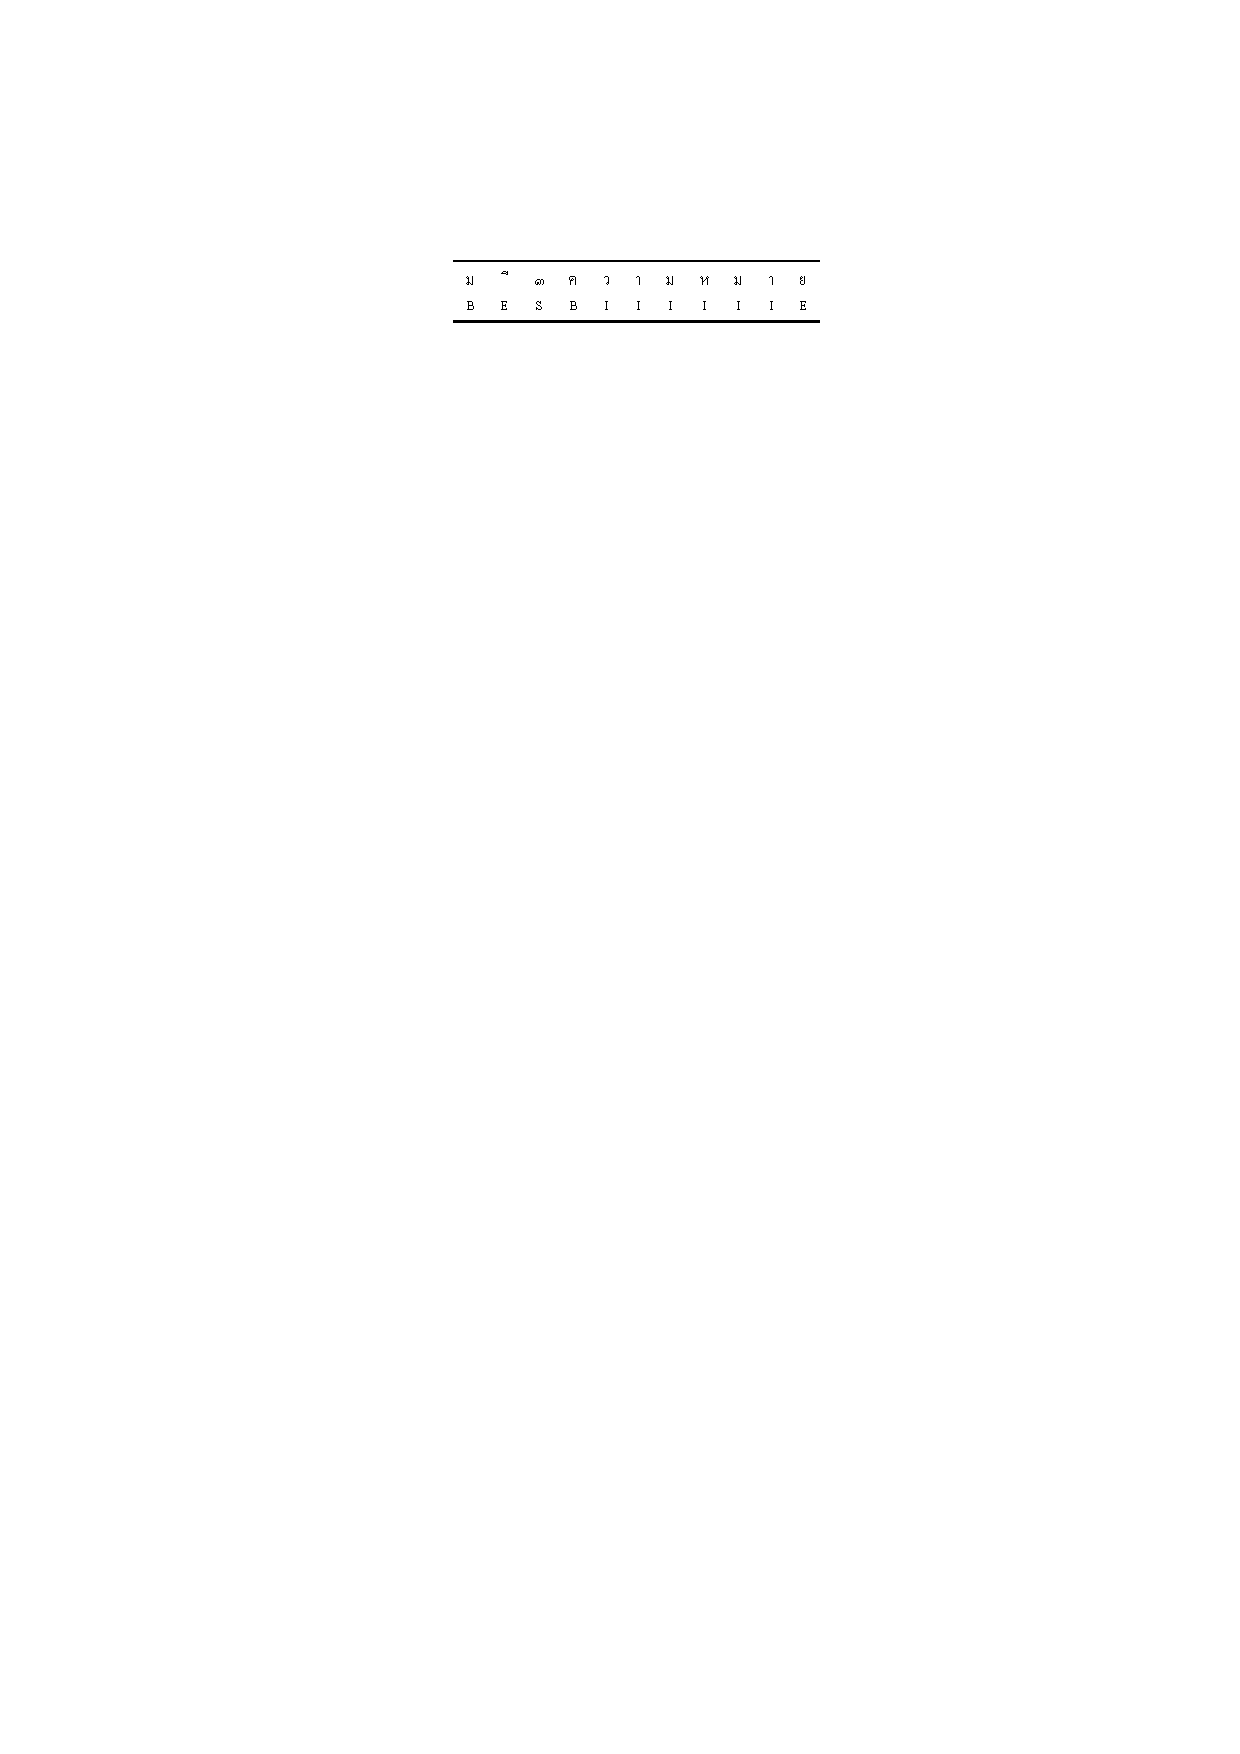
\includegraphics[width=\textwidth]{figures/fig-thbies.pdf}
    \end{subfigure}
    \hspace{\textwidth}
    \begin{subfigure}{0.24\textwidth}   
        \centering
        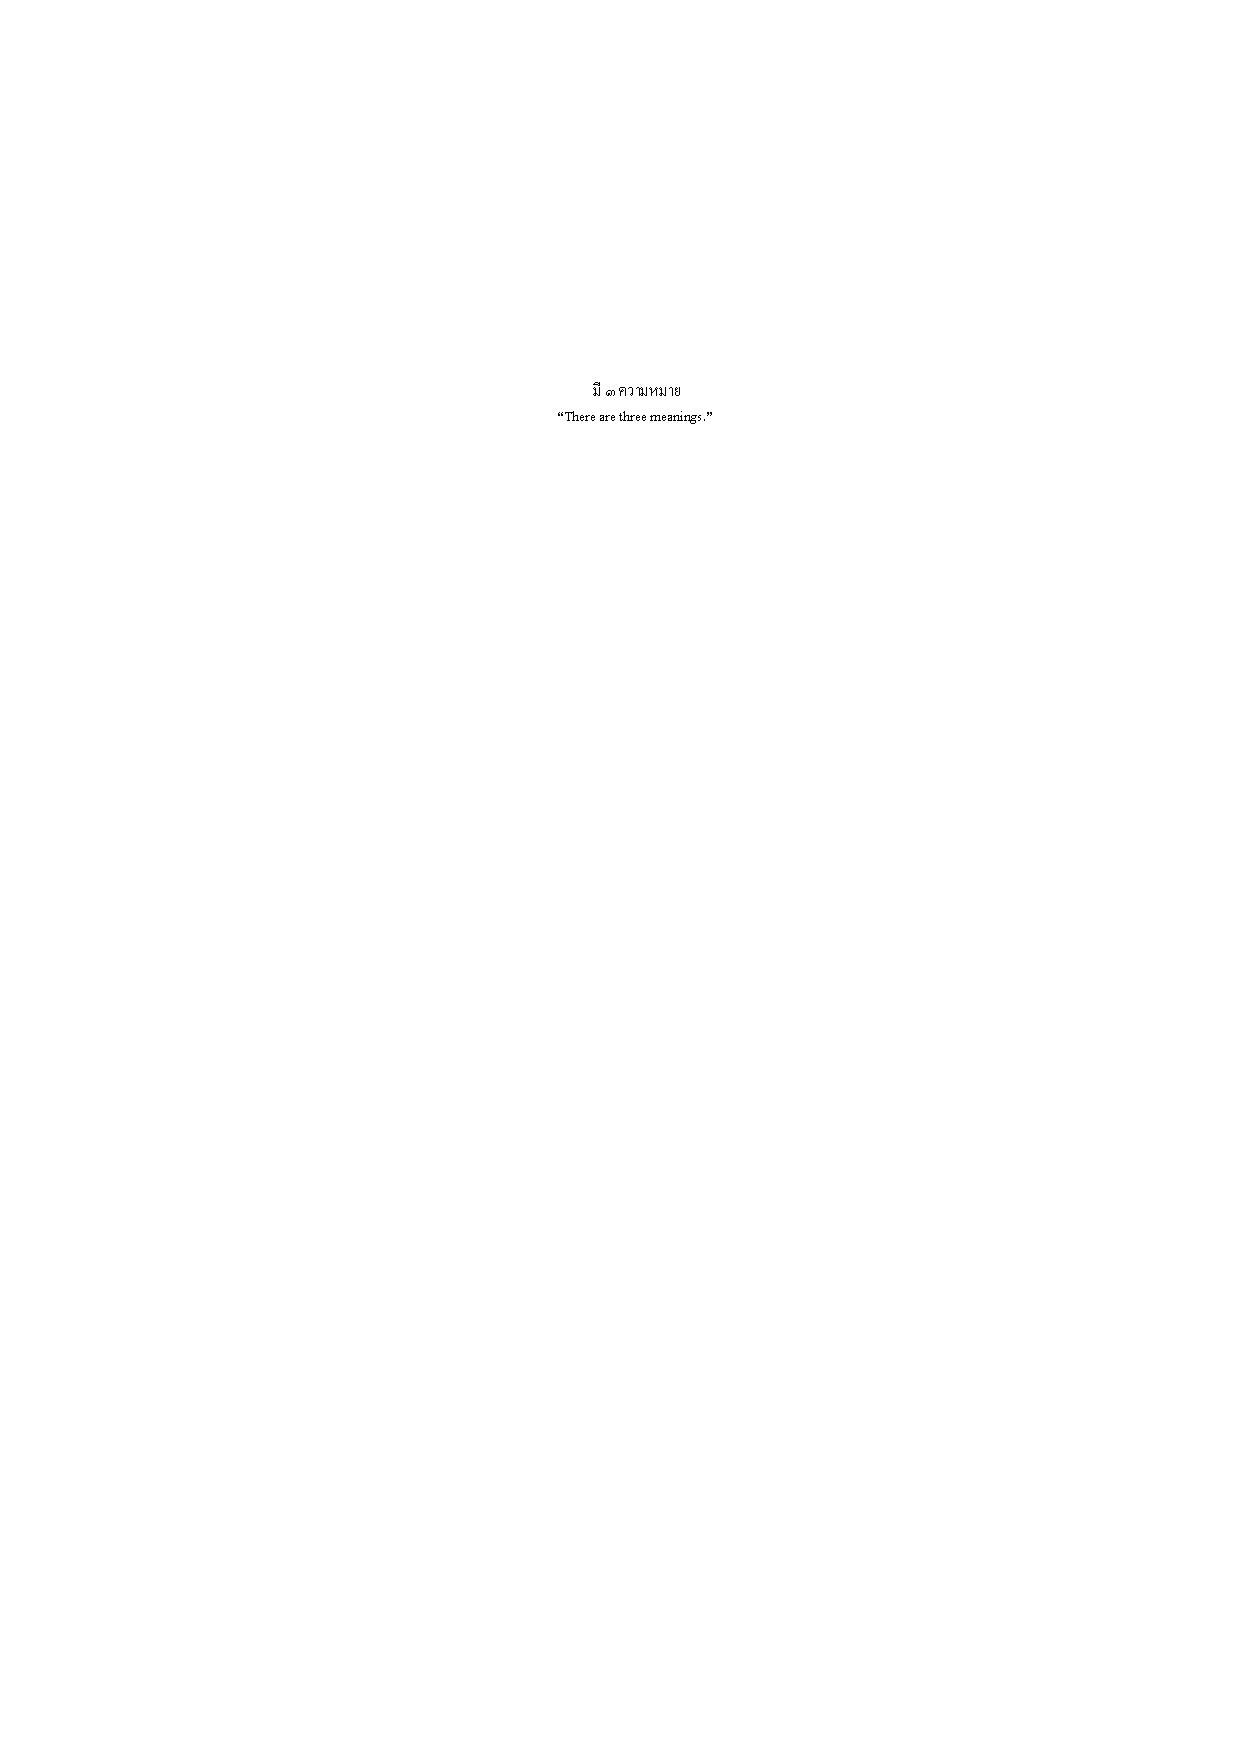
\includegraphics[width=\textwidth]{figures/fig-thbies-tran.pdf}
    \end{subfigure}
    \caption{Thai word segmentation as sequence-labeling task on BIES (beginning, inside, end, and singleton) tagging scheme.}
    \label{fig:thbies}
\end{figure}
%

Neural-network models have been applied and perform well on character-based Thai word segmentation.
%
\citeA{Jousimo2017} applied bidirectional recurrent neural networks with gated recurrent units (GRUs), while \citeA{Chormai2019} proposed an AttaCut \cite{Chormai2019},\footnote{https://github.com/PyThaiNLP/attacut} a convolutional-neural-network (CNN)-based model that mainly provides faster and more accurate word inferring motivated by DeepCut \cite{Kittinaradorn2019}.
%
% See Appendix~\ref{appx:thai-wordseg} for more details.
%
Despite the fact that neural-network models with linguistic knowledge can perform almost perfectly, adapting models with pre-trained neural networks, such as word vectors and language models, is still useful \cite{Shao2018,yan-etal-2020-bert}.
%

In spite of that a pre-trained model (PTM) such as BERT \cite{devlin-etal-2019-bert} has also been successfully applied for word segmentation mostly on Chinese datasets \cite{yang-etal-2019-bert,qiu-etal-2020-concise,ke-etal-2020-unified,huang-etal-2020-towards,ke-etal-2021-pre}, only \citeA{seeha-etal-2020-thailmcut} proposed a transfer-learning approach for Thai word segmentation by pre-training language model on the basis of character-level for character-based word segmentation. 
%
Although it exhibited state-of-the-art performance regarding Thai, it merely uses characters and does not use other information such as word and subword \cite{sennrich-etal-2016-neural,kudo-2018-subword}.
%
However, relying on the transfer-learning method can interact only input and output layers of the models, as known as black boxes, which is considered as its limitation \cite{limkonchotiwat-etal-2020-domain}. 
%
\citeA{limkonchotiwat-etal-2020-domain,limkonchotiwat-etal-2021-handling} proposed alternative approaches to particularly focus on domain-dependent word segmentation to lessen the black box limitation in the transfer learning.
%
Their works could obtain comparable results as the transfer learning method.
%

Additional linguistic-knowledge other than a character sequence, e.g., word, subword, and Thai character clusters (CCs) \cite{Theeramunkong2000} has also been successfully used for word segmentation and downstream tasks \cite{Sutantayawalee2015,Lapjaturapit2018,Nararatwong2018,yang-etal-2019-subword,li-etal-2019-word-segmentation}.
%
Furthermore, an attention mechanism \cite{Bahdanau2015} has been effectively applied to various downstream tasks, particularly a character-based sequence-labeling task that exploit more than one linguistic knowledge \cite{higashiyama-etal-2019-incorporating,tian-etal-2020-joint}.
%

To exploit multiple linguistic-knowledge, we propose a character-based Thai word-segmentation model with multiple attentions that jointly uses corresponding words, CCs, and subwords.
%
Our model is based on the bidirectional long short-term memory with conditional random field (BiLSTM-CRF) architecture, which is the baseline model for this study, because it has been successfully applied in sequence-labeling tasks for Thai and other languages \cite{Jousimo2017,Nararatwong2018,higashiyama-etal-2019-incorporating,seeha-etal-2020-thailmcut,tian-etal-2020-joint}.

%
Furthermore, Transformer-based PTM has not been incorporated in Thai word segmentation.
%
Thus, we additionally expand potential of using a pre-trained model, particularly Transformer-based PTM, in Thai word segmentation by applying BERT into our model.
%
To our best knowledge, this work is the first to adopts PTM in Thai word segmentation. 

Our contributions are as follows:
%
\begin{itemize}
    \setlength\itemsep{0.01em}
    \item We use word, CC, and subword with multiple attentions to estimate the relationships of characters in character-based Thai word segmentation.
    \item We conduct experiment for showing the validity of using CC over subword units in terms of segmentation performance and a segmentation result that does not violate Thai writing system.
    \item Our model shows improvement over the baseline model and outperforms previous works in Thai word segmentation.
    \item Our proposed model outperforms recent works that focus domain-dependent word segmentation on Thai domain-dependent datasets.
    \item We incorporate Multilingual BERT into character-based Thai word segmentation, and conduct a comparison between our BiLSTM-based model and BERT-based model. Moreover, we found that most of BERT-incorporated model could not outperform our proposed BiLSTM-based model.
    \item Our code is publicly available.\footnote{\url{https://github.com/tchayintr/thwcc-attn}}
\end{itemize}